\section{Матрица Кирхгофа, ее применение для нахождения числа остовных деревьев. Корневые деревья: 
основные определения. Найти число остовных деревьев с помощью матрицы Кирхгофа.}

Пусть $G$ -- связный неориентированный граф. $|V| = n$.

\begin{definition}
    \textit{Матрицей Кирхгофа} графа $G$ называется квадратная матрица
    размерности $n \times n$, в которой
    \begin{align*}
        b_{ij}&=\begin{cases}
            k,&  \text{где $\delta(v_i)=k, i=j$},\\
            -1,& \text{если $i \neq j$, $v_i$ и $v_j$ смежны}, \\
            0,&  \text{если $v_i$ и $v_j$ не смежны}.
            \end{cases}
    \end{align*}
\end{definition}

\begin{theorem}
    Число остовных деревьев в связном графе $G$, равно алгебраическому
    дополнению любого элемента матрицы Кирхгофа.
\end{theorem}

Пример. Изобразить граф, заданный с помощью матрицы Кирхгофа, найти
число остовных деревьев графа и их изобразить.
\begin{figure}[h]
    \centering
    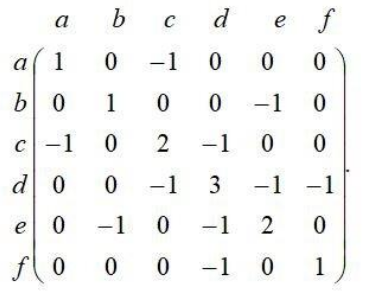
\includegraphics[scale=0.4]{26.png}
\end{figure}

Найдем алгебраическое дополнение элемента матрицы с индексом 44.

$A_{44} = 1$. Это означает, что существует лишь одно остовное дерево этого графа.
Это остовное дерево является самим графом.

\newpage
\textbf{Корневые деревья}
\begin{definition}
    \textit{Корневым деревом} называют дерево с выделенной вершиной --
    корнем.
\end{definition}

\begin{definition}
    Висячую вершину корневого дерева называют \textit{листом}.
    \textit{Высотой корневого дерева} называют расстояние от корня до самого
    удаленного листа. Если в корневом дереве маршрут, соединяющий вершину $u$
    c корнем, проходит через вершину $v$, то говорят, что вершина u -- \textit{потомок
    вершины} $v$, вершина $v$ -- \textit{предок вершины} $u$. Множество всех потомков
    вершины $v$ является деревом с корнем $v$, оно называется \textit{ветвью дерева} в
    вершине $v$. Если предок и потомок соединены ребром, то они называются
    \textit{отцом и сыном}.
\end{definition}

На рисунке пример дерева, в котором выделили вершину $v_4$ и оно стало
корневым деревом. Обычно корень принято изображать сверху (как в
генеалогическом древе). Иногда его изображают внизу.

\begin{figure}[h]
    \centering
    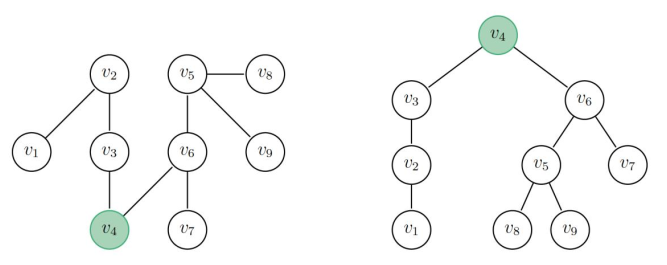
\includegraphics[scale=0.4]{26_2.png}
\end{figure}

У графа на рисунке высота корневого дерева равна трем.

Для вершин $v_1$ и $v_3$, вершина $v_1$ -- \textit{потомок} вершины $v_3$, вершина $v_3$ \textit{предок}
вершины $v_1$, вершина $v_2$ -- \textit{отец} вершины $v_1$.

Множество вершин $\set{v_1, v_2, v_3}$ всех потомков вершины $v_3$ является деревом с
корнем $v_3$, оно является ветвью дерева в вершине $v_3$.

\begin{definition}
    Ориентированным деревом называют ориентированный граф
    без циклов, в котором в каждую вершину, кроме одной, называемой корнем,
    входит ровно одно ребро. В корень ориентированного дерева не входит ни
    одного ребра.
\end{definition}

Иногда ориентированные деревья изображают с вершиной -- корнем
внизу, ребра также могут быть изображены направленными в сторону корня.